\documentclass[11pt,a4paper]{scrartcl}
\usepackage[T1]{fontenc}
\usepackage[utf8]{inputenc}
%\usepackage[ngerman]{babel}
\usepackage[ngerman,english]{babel}
\selectlanguage{english}
\usepackage{microtype}
\usepackage{lmodern}
\usepackage{amsmath}
\usepackage{amsfonts}
\usepackage{amssymb}
\usepackage{enumerate}
\usepackage{graphicx}
\usepackage{listings}
\usepackage{color}
\usepackage{url}
\usepackage{multicol}
\usepackage{wrapfig}
\usepackage{amsmath}
\usepackage{tikz}
\usetikzlibrary{arrows}


\begin{document}

\author{Ralf Vogler}
\title{Program Optimization}
\subtitle{Exercise sheet 10}

\maketitle

\section*{Exercise 1: Live ranges \& interference graph}
\begin{minipage}[t]{0.5\textwidth}
\subsection*{a) True liveness}
\begin{tabular}{|c|c|}
\hline
& $\mathcal{L}$ \\
\hline
7 & $\emptyset$ \\
5 & $\{r\}$ \\
6 & $\{y\}$ \\
4 & $\{x\}$ \\
3 & $\{x, y\}$ \\
2 & $\{r, y\}$ \\
1 & $\{r\}$ \\
\hline
\end{tabular}
\end{minipage}
\begin{minipage}[t]{0.5\textwidth}
\subsection*{b) Live ranges}
\begin{tabular}{|c|c|}
\hline
x & \{3, 4\} \\
y & \{2, 3, 6\} \\
r & \{1, 2, 5\} \\
\hline
\end{tabular}
\end{minipage}

\subsection*{c) Interference graph}
\begin{tikzpicture}[,shorten >=1pt,auto,node distance=1.8cm,
  thick,main node/.style={circle, fill=blue!20,draw,font=\sffamily\Large\bfseries}]

  \node[main node] (1) {x};
  \node[main node] [below left of=1] (2) {y};
  \node[main node] [below right of=1] (3) {r};

  \path[every node/.style={font=\sffamily\small}]
    (1) edge node {} (2)
    (2) edge node {} (3);
\end{tikzpicture}

\subsection*{d) Color graph using greedy heuristic}
Order of colors: red, green, blue
\begin{enumerate}
\item Start with node x, smallest color is red
\item Smallest color, different from self and colored neighbours is green
\item Color uncolored neighbours -> y becomes green
\item Next uncolored node is r, smallest unconnected color is red
\end{enumerate}
\begin{tikzpicture}[,shorten >=1pt,auto,node distance=1.8cm,
  thick,main node/.style={circle, fill=blue!20,draw,font=\sffamily\Large\bfseries}]

  \node[main node] [fill=red] (1) {x};
  \node[main node] [fill=green, below left of=1] (2) {y};
  \node[main node] [fill=red, below right of=1] (3) {r};

  \path[every node/.style={font=\sffamily\small}]
    (1) edge node {} (2)
    (2) edge node {} (3);
\end{tikzpicture}

\subsection*{e) Interval graph, live range splitting}
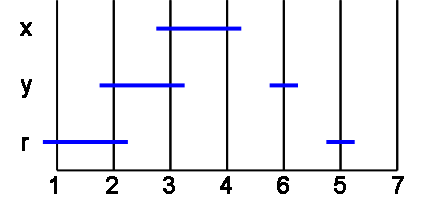
\includegraphics[scale=.8]{1e}\\
From 1 to 4 the intervals of r, y and x interfere and therefore have to stay together.
After that, the live ranges of y and r can be split at 6 and 5 (named $y_1$ and $r_1$).

\subsection*{f) Interference graph where live ranges have been split}
\begin{tikzpicture}[,shorten >=1pt,auto,node distance=1.8cm,
  thick,main node/.style={circle, fill=blue!20,draw,font=\sffamily\Large\bfseries}]

  \node[main node] (1) {x};
  \node[main node] [below left of=1] (2) {y};
  \node[main node] [below right of=1] (3) {r};

  \path[every node/.style={font=\sffamily\small}]
    (1) edge node {} (2)
    (2) edge node {} (3);
\end{tikzpicture}
\hspace{2cm}
\begin{tikzpicture}[,shorten >=1pt,auto,node distance=1.8cm,
  thick,main node/.style={circle, fill=blue!20,draw,font=\sffamily\Large\bfseries}]

  \node[main node] (1) {$y_1$};
  \node[main node] [below of=1](2) {$r_1$};
\end{tikzpicture}

\subsection*{g) Color graph using greedy heuristic}
The order is the same as in d). Since $y_1$ and $r_1$ are seperate unconnected components now, they each get the smallest color.\\
\begin{tikzpicture}[,shorten >=1pt,auto,node distance=1.8cm,
  thick,main node/.style={circle, fill=blue!20,draw,font=\sffamily\Large\bfseries}]

  \node[main node] [fill=red] (1) {x};
  \node[main node] [fill=green, below left of=1] (2) {y};
  \node[main node] [fill=red, below right of=1] (3) {r};

  \path[every node/.style={font=\sffamily\small}]
    (1) edge node {} (2)
    (2) edge node {} (3);
\end{tikzpicture}
\hspace{2cm}
\begin{tikzpicture}[,shorten >=1pt,auto,node distance=1.8cm,
  thick,main node/.style={circle, fill=blue!20,draw,font=\sffamily\Large\bfseries}]

  \node[main node] [fill=red] (1) {$y_1$};
  \node[main node] [fill=red] [below of=1](2) {$r_1$};
\end{tikzpicture}



\section*{Exercise 2: SSA}
Graph with inserted $\psi$ -edges:\\
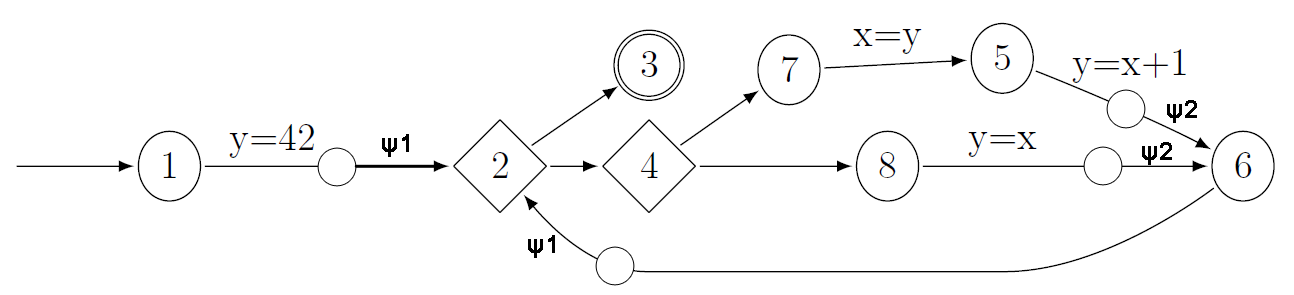
\includegraphics[scale=.35]{2a}\\
Reaching definitions:\\
\begin{tabular}{|c|c|}
\hline
& $\mathcal{R}$ \\
\hline
1 & <x, 1>, <y, 1> \\
2 & <x, 1>, <x, 5>, <y, 2>, <y, 6> \\
3 & <x, 1>, <x, 5>, <y, 2>, <y, 6> \\
4 & <x, 1>, <x, 5>, <y, 2>, <y, 6> \\
7 & <x, 1>, <x, 5>, <y, 2>, <y, 6> \\
8 & <x, 1>, <x, 5>, <y, 2>, <y, 6> \\
5 & <x, 5>, <y, 2>, <y, 6> \\
6 & <x, 1>, <x, 5>, <y, 6> \\
\hline
\end{tabular}\\
\begin{align*}
\psi_1 = x = x | y = y \\
\psi_2 = x = x | y = y
\end{align*}

Renamed:\\
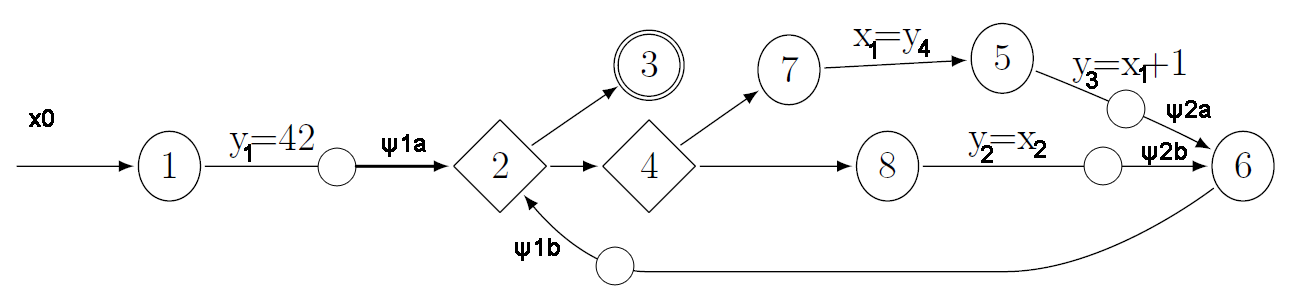
\includegraphics[scale=.35]{2b}\\
\begin{align*}
\psi_1a = x_2 = x_0 | y_4 = y_1 \\
\psi_2a = x_2 = x_1 | y_4 = y_3 \\
\psi_2b = x_2 = x_2 | y_4 = y_2 \\
\psi_1b = x_2 = x_2 | y_4 = y_4 \\
\end{align*}

\end{document}

















